\documentclass[a4paper,12pt]{article}

\usepackage{graphicx}
\usepackage{float}
\usepackage{amsmath}

\usepackage[hyphens]{url}
\usepackage[margin=1.2in]{geometry}

\usepackage{subcaption}
\usepackage[title,titletoc,page]{appendix}

\usepackage{titlesec}
\titlespacing*{\section}
{0pt}{5.5ex plus 1ex minus .2ex}{5.3ex plus .2ex}
\titlespacing*{\subsection}
{0pt}{5.5ex plus 1ex minus .2ex}{4.3ex plus .2ex}

\author{\vspace{1cm} \\
        Christopher Brown (2077762) \\
        Jack Croal (2062685) \\
        Cameron Houston (2082989) \\
        Alex Smith (2083008) \\
        Jok\=ubas Surgailis (2065915) \\
}

\date{}

\title{\vspace{1.0cm}Steering Wheel Display - Final Report\vspace{1.0cm}}

\setlength\parindent{0pt}
\newcommand{\forceindent}{\leavevmode{\parindent=6em\indent}}

\begin{document}

\maketitle

\thispagestyle{empty}

\begin{center}
\Large{Team Project EE4}
\end{center}

\begin{center}
\huge{Team VoltsWagen}
\end{center}

\vspace{2.0cm}

\begin{center}

\includegraphics[width=8cm]{Figures/uni_logo.png}

\includegraphics[width=8cm]{Figures/ugr_logo_black.png}
\end{center}

\clearpage
\pagenumbering{arabic}

% TODO: figure out how to include code
% TODO: plaigiarism check

% ====================================================================================================================

\newpage
{\Huge Acknowledgements} \\

{\large

  \vspace{1.0cm}

  Team VoltsWagen would like to thank the following people for their advice and counselling over the course of the project. \\

  \vspace{1.0cm}

  \center{
    Dr David Muir
  }
  \center{
    Mr Andrew Phillips
  }
  \center{
    Dr Jon Trinder
  }
  \center{
    Mrs Shona Ballantyne
  }

}

% ====================================================================================================================

\newpage
\tableofcontents

% ====================================================================================================================

\newpage
\section{Introduction}
\label{sec:introduction}

As part of the Glasgow University Team Project EE4 course, a steering wheel display has been designed and prototyped for use within a University of Glasgow Racing (UGR) car. UGR is the Glasgow University engineering team competing in Formula Student. Formula Student is a competition inspiring University students to design and build a single-seat race car. Each team’s race car is then put to the test against other teams from around the world. The Formula Student 2017 competition takes place on the 20th July 2017 at Silverstone Circuit, England. \\

This display allows the driver of the car to view live information from the CAN bus about the current status of the car. It is important for the UGR race car driver to be able to view the information concerning the status of the race car because this allows the driver to understand how the car is performing. A regular car dashboard would not suit a racing environment because only specific information should be shown to the driver and there is limited space with the confines of the car `cockpit'. In order for the driver to be able to view this status information, a small display is required. This display would show the car status information such as the speed, RPM, gear number and coolant temperature by attaching directly to the car’s steering wheel. The values of these indicators were to be retrieved from the car's central CAN (Controller Area Network) bus (See Section \ref{sec:device_overview}). \\

Being the main client for the project, UGR were involved throughout the design and manufacturing of the final product. The following report covers the requirements and specifications of the completed steering wheel display, describing in detail each component and the reasons for the design. \\

\begin{figure}[H]
\begin{center}
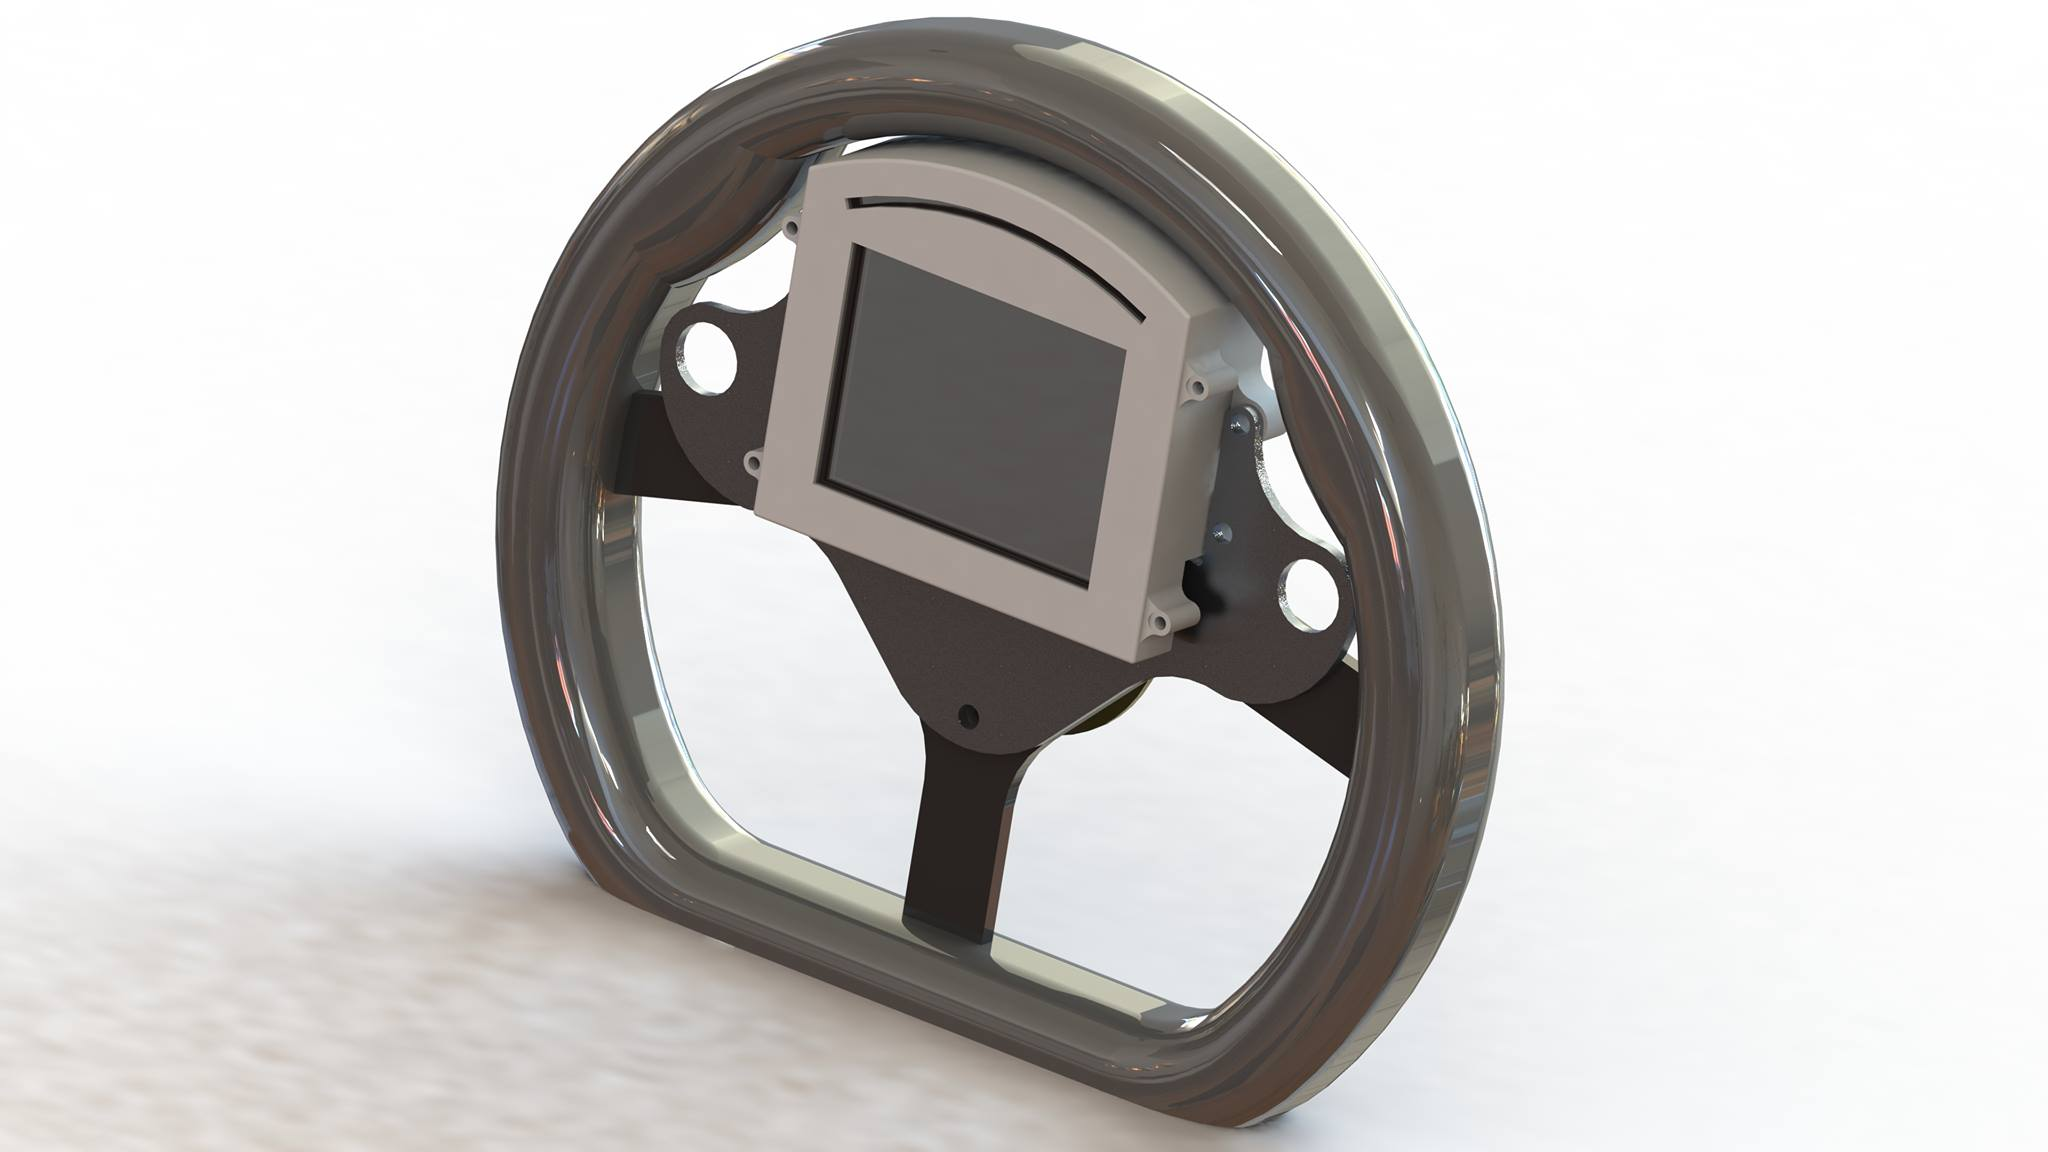
\includegraphics[width=12cm]{Figures/device_render_wheel.jpg}
\end{center}
\caption{SolidWorks render of outer enclosure attached to steering wheel}
\label{fig:device_render_wheel}
\end{figure}


% ====================================================================================================================

\newpage
\section{Device Requirements}
\label{sec:device_requirements}

This section covers the overall requirements for the device. These requirements were obtained from the UGR team. \\

The device was required to display the following status indicators to the driver:

\begin{enumerate}
  \item Speed (MPH).
  \item Gear number (including `Neutral').
  \item Coolant temperature.
  \item Engine RPM.
  \item Battery Voltage.
  \item Coolant threshold warning symbol.
\end{enumerate}

In order to function properly, certain aspects of these displayed values were required to be configurable by the user. This would increase the portability and flexibility of the device. The specific details of the configurability are described further in Section \ref{sec:configuration_software}. \\

The device had to be attachable to the steering wheel. This introduced a size constraint on the overall device. The size constraint provided by the UGR team is that the device needed to fit within 116mm x 70mm x 20mm. This would allow the device to fit within the steering wheel, and not get in the way of the driver. \\

\textbf{Waterproofing} \\

It was required of the device to be IP67 compliant. This specifies that the device had to be waterproof to 1m, and fully dustproof. This was because the steering wheel display needed to be operational in poor weather conditions. \\

\textbf{Reliability} \\

The device was to be used in a mechanical environment, and therefore needed to be sturdy. It also had to be resistant to high voltage spikes on the outside connections. \\

\textbf{Overheating} \\

The heat budget for the device was also important. The device was to be used for long periods of time on the race track, possibly in warm temperatures. As a result, sufficient precautions for the disipation of heat and the reduction of heat generation from the device needed to be taken.

% ====================================================================================================================

\newpage
\section{Device Overview}
\label{sec:device_overview}

The device consisted of four main components: the RPM LEDs, the microcontroller, the LCD screen and the CAN bus electronics. Figure \ref{fig:block_diagram} shows the overall block diagram of the device. \\

\begin{figure}[H]
\begin{center}
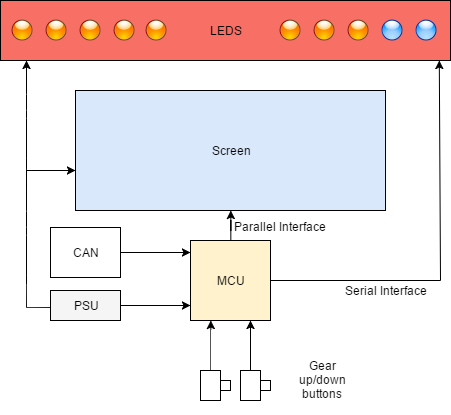
\includegraphics[width=12cm]{Figures/refined_block_diagram.png}
\end{center}
\caption{High level device block diagram.}
\label{fig:block_diagram}
\end{figure}


CAN bus is a serial communication technology used with motor vehicles to send information between individual systems and sensors. The car's central CAN bus was used to transmit the display information to the microcontroller and supply the device with power ($\sim$ 12 V DC). \\

The microcontroller would then process the data and output it the format required for the LCD display and RPM LEDs. \\

% ====================================================================================================================

\newpage
\section{Electrical Design}
\label{sec:electrical_design}

When selecting components for the final device, each component was evaluated individually and in detail. In order to aid the construction process, each component needed to be in stock and readily available from a trusted distributor. The following section describes the requirements and final decisions for each component within the steering wheel display device. \\

The full circuit diagram is included in Appendix \ref{app:circuit_diagram}.

\subsection{Microcontroller Requirements and Selection}
\label{sec:microcontroller}

The microcontroller was to be chosen to minimise the number of peripheral elements required, whilst exhibiting sufficient processing power and I/O bus speed to provide to the LCD display, LEDs and other peripherals. As a result, the microcontroller was required to include:

\begin{enumerate}
  \item Sufficient number of digital output pins.
  \item CAN module.
  \item Fast digital I/O to update LCD display rapidly.
  \item Sufficient on-board memory.
\end{enumerate}

The microcontroller also had to be available in a package that could be soldered by hand. \\

Built-in writable flash memory was also required on the microcontroller so that state could be stored when turning the device on and off. The flash memory was to be used to store configuration details that were programmable by the user. A software description for this feature is detailed in Section \ref{sec:CAN_software}. \\

The Atmel SAM3X8E ARM Cortex-M3 microcontroller was selected for the device \cite{microcontroller}. This microcontroller is used in the Arduino Due boards. The decision to make use of an Arduino-integrated microcontroller was based upon the ease of use and vast quantity of Arduino platform packages, libraries and support available. The Arduino Due was used as a basis for much of the design of the steering wheel display circuitry, and also for early prototyping. The Quad Flat Package version was selected to allow for ease of soldering. \\

The Atmel SAM3X8E also included 2 CAN modules. This was useful because it allowed the testing of the CAN software without the use of more than one microcontroller; the microcontroller could send and receive to itself. \\

\subsection{LCD Display Requirements and Selection}
\label{sec:display}

The LCD display was to be used to display the majority of the car information to the driver, so it was very important for it to be able to display the appropriate information clearly and reliably. The requirements outlined by UGR are as follows:

\begin{enumerate}
  \item Clearly visible even in direct sunlight: brightness over 250 cd/$\textrm{m}^2$.
  \item Large enough to display all required information clearly.
  \item Easy to read at a glance.
  \item Available in a thin package, to reduce the depth of the device.
\end{enumerate}

As well as the operational requirements listed above, further requirements were included by the VoltsWagen team in order to ensure the functionality of the device. This included a built-in display controller to make the software less complex and easier to write. This would allow the microcontroller to communicate with the display via the controller, instead of addressing individual registers on the display. Secondly, the team required clearly documented controller code to assist with programming. Lastly, as a result of the mechanical design of the outer enclosure, the display required metal or plastic tabs to allow it to fit properly within the device. \\

As a result of the requirements, the MIDAS MCT035AB0W320240LML TFT LCD display was selected \cite{display_datasheet}. This is a 320 x 240 pixel display, with a screen size of 3.5" and an input voltage of 3.3 V. The package size was 93.5mm x 66.44mm x 7.3mm, which would allow the screen to fit within the space requirements of the outer enclosure. The display fitted all of the requirements given.

\subsection{RPM Gauge Requirements and Selection}
\label{sec:LEDs}

In order to display the engine RPM of the car more clearly, coloured LEDs were a requirement given by the client. These LEDs were to be above the screen and had to be easy to read even in direct sunlight. The client preferred to use different colours of LEDs, depending on how high the engine RPM was. \\

It was decided to use Adafruit DotStar LEDs for the RPM indicator \cite{dotstar_datasheet}. These devices use 2-wire SPI daisy-chain configuration which allow the programmer to configure the brightness and colour of individual LED’s in the strip. This is accomplished with an embedded LED driver chip within the DotStar package. Because the LEDs could be controlled with only 2 wires, the amount of wiring required was reduced. A simplified circuit diagram of the DotStar LEDs is shown in Figure \ref{fig:leds_4}. The Data In (DI) and Clock (Cl) pins are shown being input to the first LED, which is then connected to the rest of the chain.

\begin{figure}[H]
\begin{center}
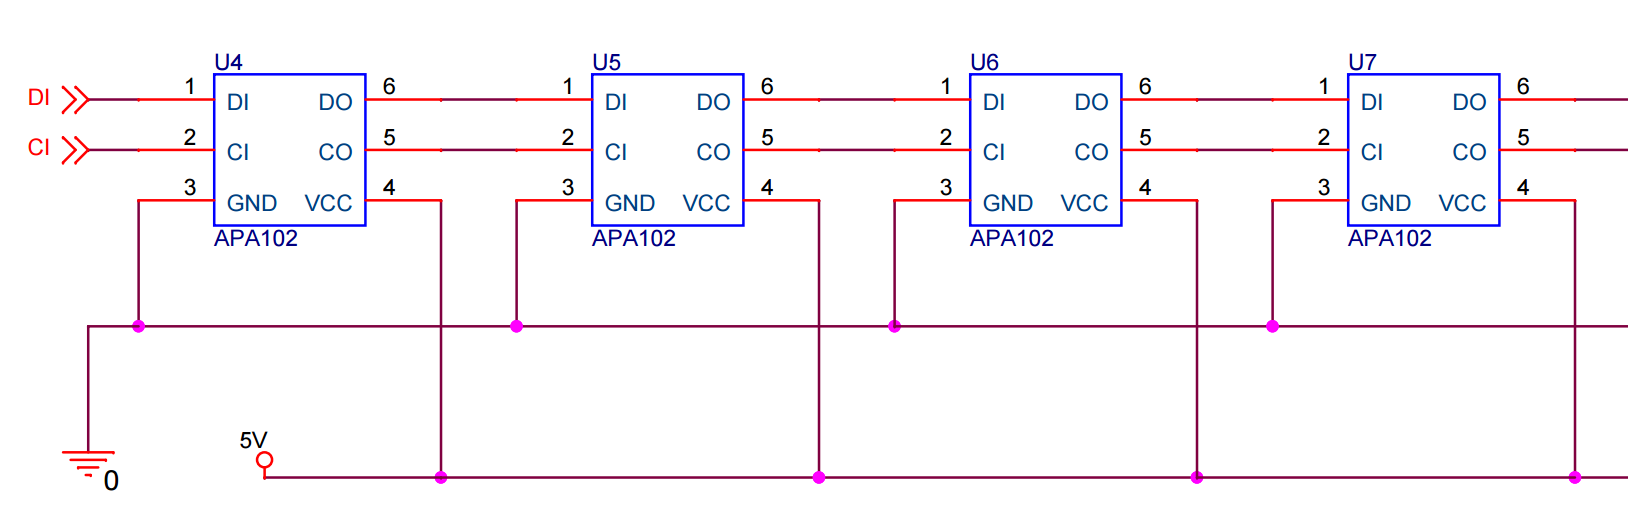
\includegraphics[width=14cm]{Figures/leds_4.png}
\end{center}
\caption{Simplified circuit diagram of LEDs.}
\label{fig:leds_4}
\end{figure}


After reviewing steering wheel display implementations from previous official Formula One racing cars, it was decided to use a three colour scheme of Green, Red, and Blue, in order of increasing RPM \cite{bsim_racing, daily_mail_1}. This ensured the device complied with the current trends in high-end steering wheel display design. Figure \ref{fig:full_leds} shows the final DotStar LEDs at full engine RPM.

\begin{figure}[H]
\begin{center}
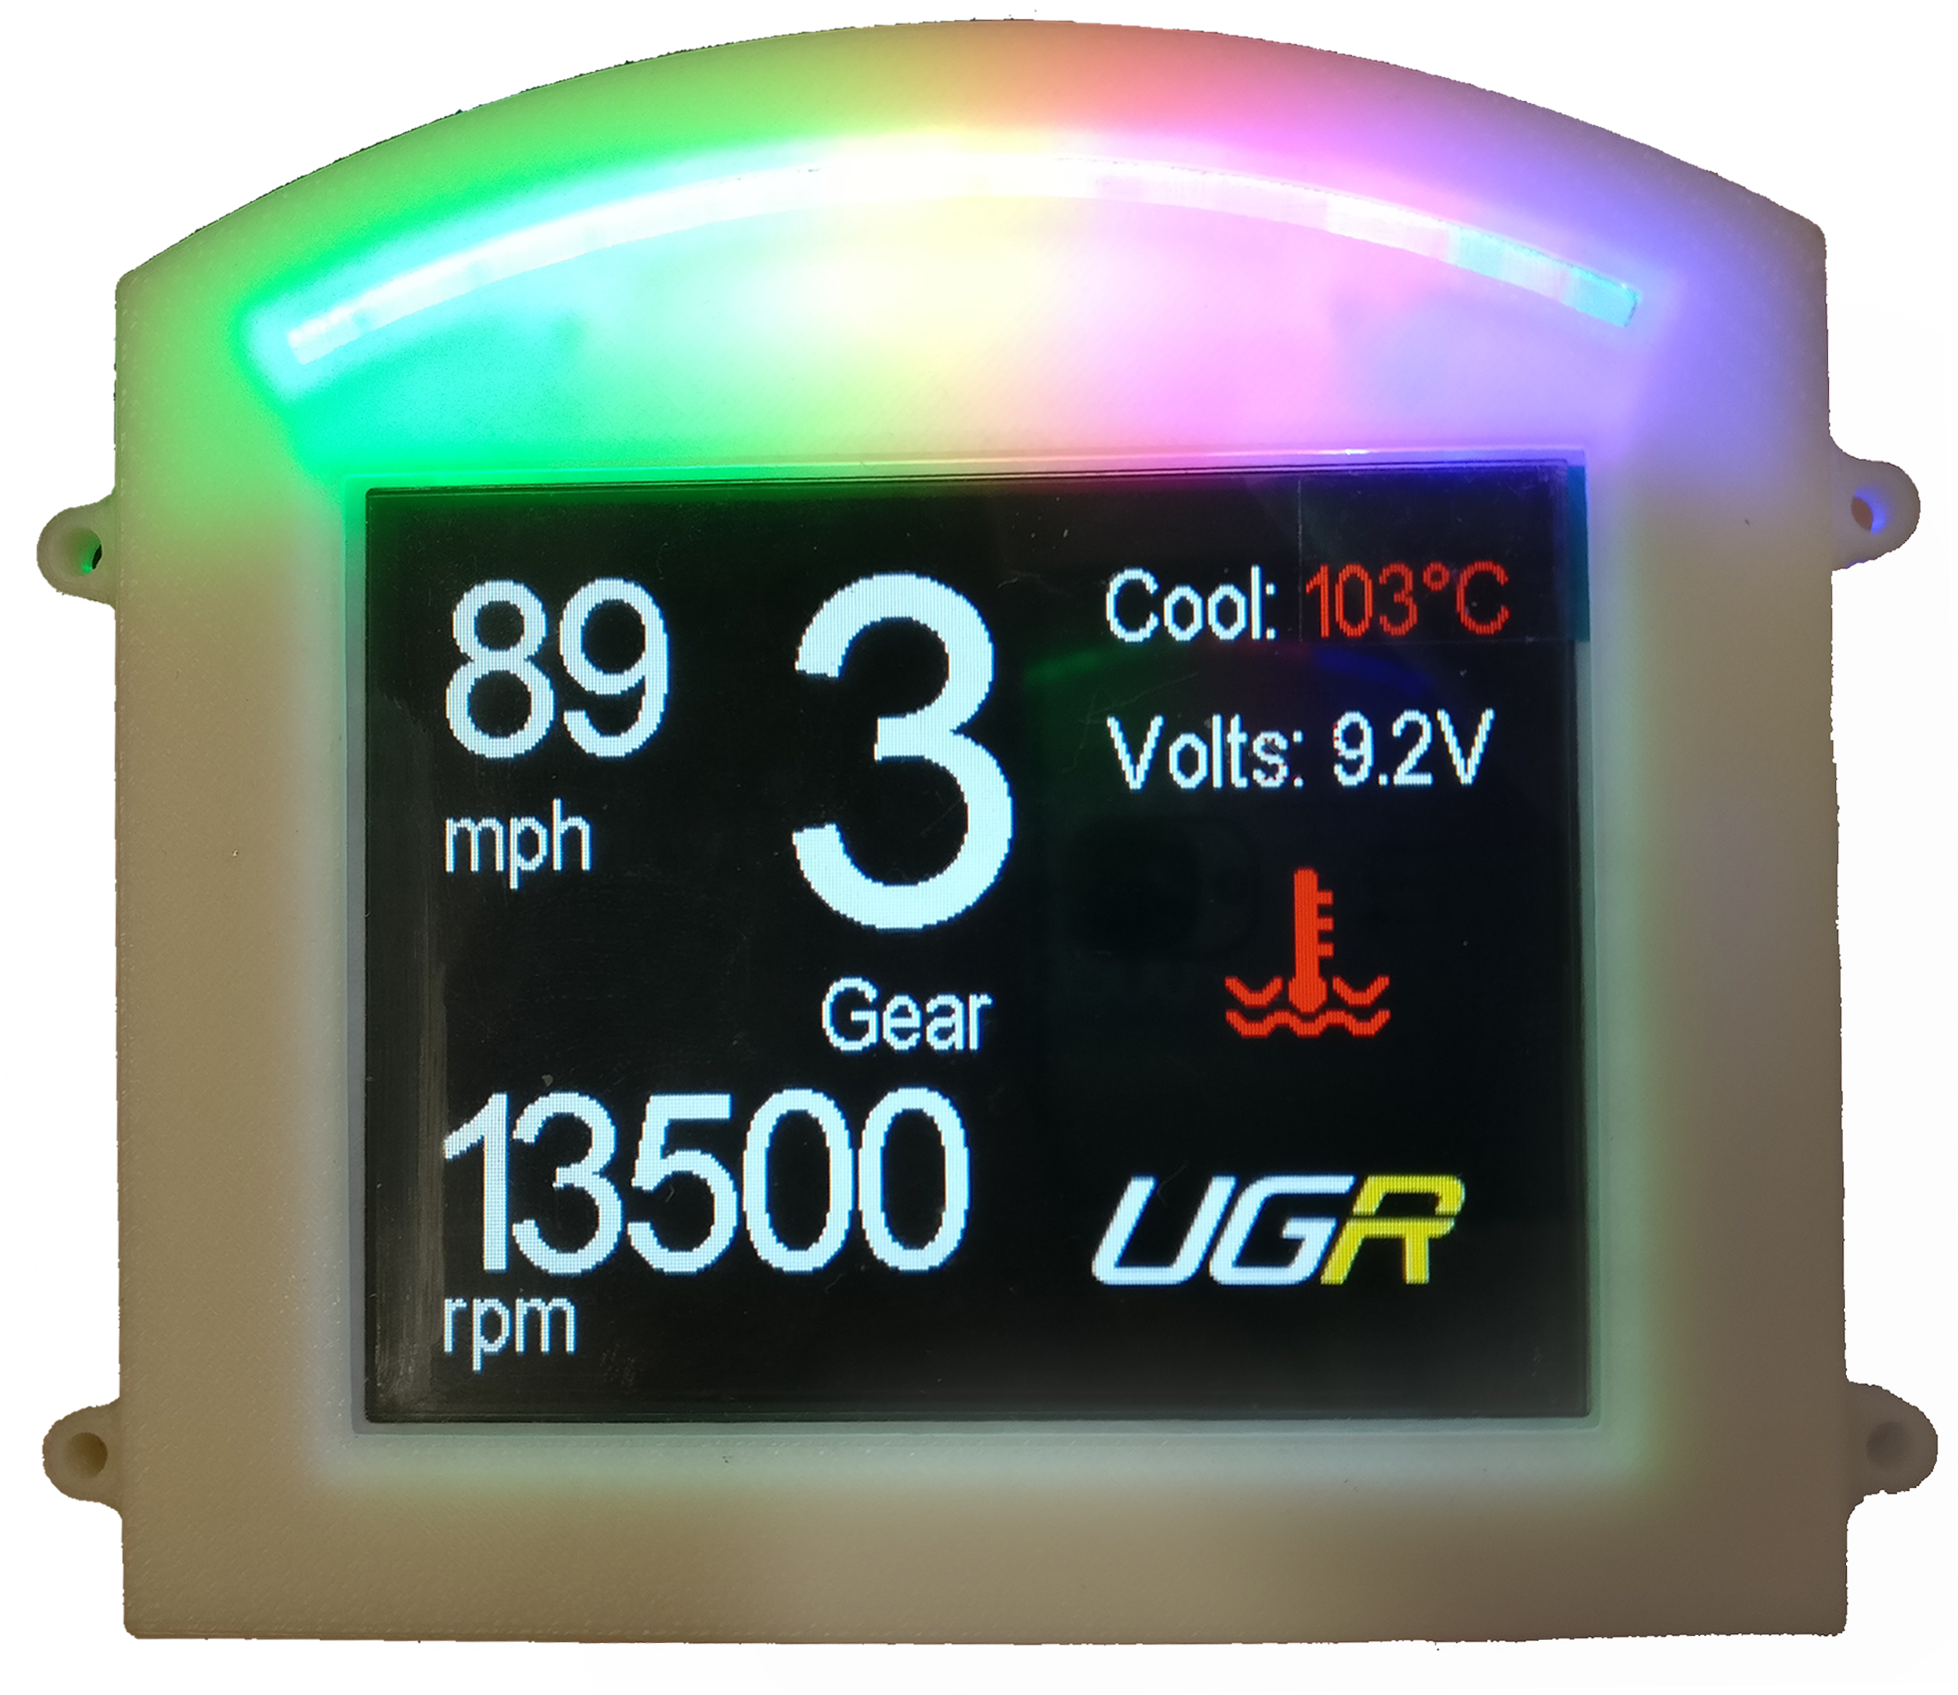
\includegraphics[width=10cm]{Figures/full_leds.png}
\end{center}
\caption{LEDs displaying at full rpm.}
\label{fig:full_leds}
\end{figure}


\newpage
\subsection{Power Supply Unit Requirements and Selection}
\label{sec:PSU}

Once the main components were selected, the overall power consumption of the device was then evaluated. Table 1 shows the calculated expected power requirements of the main components within the device. These values were obtained from the values quoted on the datasheets of each component.

\begin{center}
\begin{tabular}{ | c | c | c | c | c | c | }
\hline
 Component & Voltage (V) & Current (A) & Quantity & Power Consumption (W) \\
\hline
 LCD Display & 3.3 & 0.525 & 1 & 1.73 \\
\hline
 Microcontroller & 3.3 & 0.8 & 1 & 2.64 \\
\hline
 LEDs & 5 & 0.02 & 12 & 1.20 \\
\hline
\end{tabular}
\par
\bigskip
Table 1: Expected Power Consumption of Device. \footnote{Each DotStar was quoted to use 0.06 A with the LED on full RGB, however only one colour was to be used at a time, so a maximum of 0.02 A would be sourced.}
\end{center}

This gave an approximate total expected power of: $5.6\, W$ \\

The components were to be housed in a closed container. The generated heat needed to be controlled to ensure that the final product would not overheat in its environment. \\
 
Two regulators were required in order to step-down the 12 V DC voltage from the CAN bus to 5 V and 3.3 V power lines. The 5 V power line was used to power the RPM LEDs and the CAN bus transceiver. The 3.3 V power line was used to power the microcontroller and LCD display. Linear regulators could have been used for the voltage conversion, however these are inefficient and would have required a large heat sink in order to prevent the device from overheating. A heat sink would not be able to fit within the size requirements of the outer enclosure. Therefore, it was decided to use adjustable switching buck regulators. Specifically, the TPS563209DDCT and TPS562201DDCT regulators were selected \cite{psu_1, psu_2}. These regulators were chosen because they exhibit a very high efficiency, so a heat sink was not necessary in order to dissipate the heat. The regulators were available in a small package, and were easily configurable to allow the voltages to be fine-tuned. The Power Supply Unit (PSU) circuit diagram is shown in Figure \ref{fig:psu}.

\begin{figure}[H]
\begin{center}
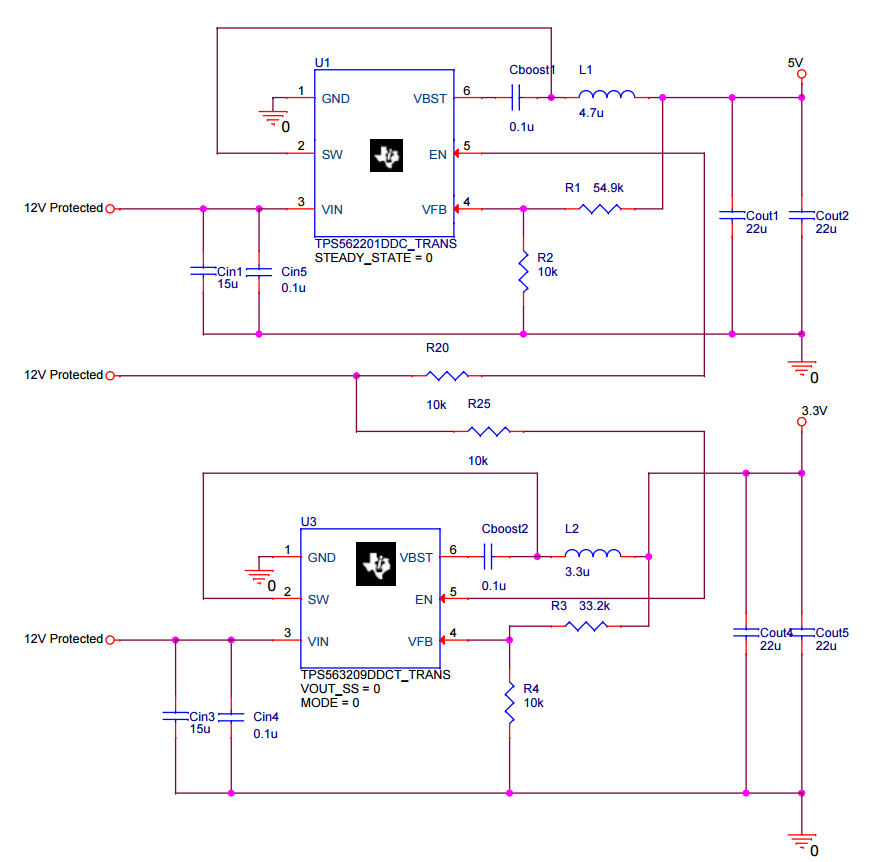
\includegraphics[width=16cm]{Appendices/psu.png}
\end{center}
\end{figure}

 
After completion, the power requirements of the device were tested in a laboratory setting. It was found that the device sourced a maximum of 0.3 A at 12 V supply voltage (3.6 W). This was a lower power value than calculated during the design phase. This result may make the device more resilient to overheating.

\newpage
\subsection{CAN Requirements and Selection}
\label{sec:CAN}

A CAN bus transceiver was used to convert the 5 V data lines of the CAN bus to the required 3.3 V input lines to the microcontroller, as well as minimising any noise. The MCP2562-E/SN was selected which came in a very small package, in order to fit within the printed circuit board (PCB) \cite{can_transciever}. Figure \ref{fig:can} shows the circuit diagram for the CAN setup, as well as the button inputs for use with the microcontroller. 

\begin{figure}[H]
\begin{center}
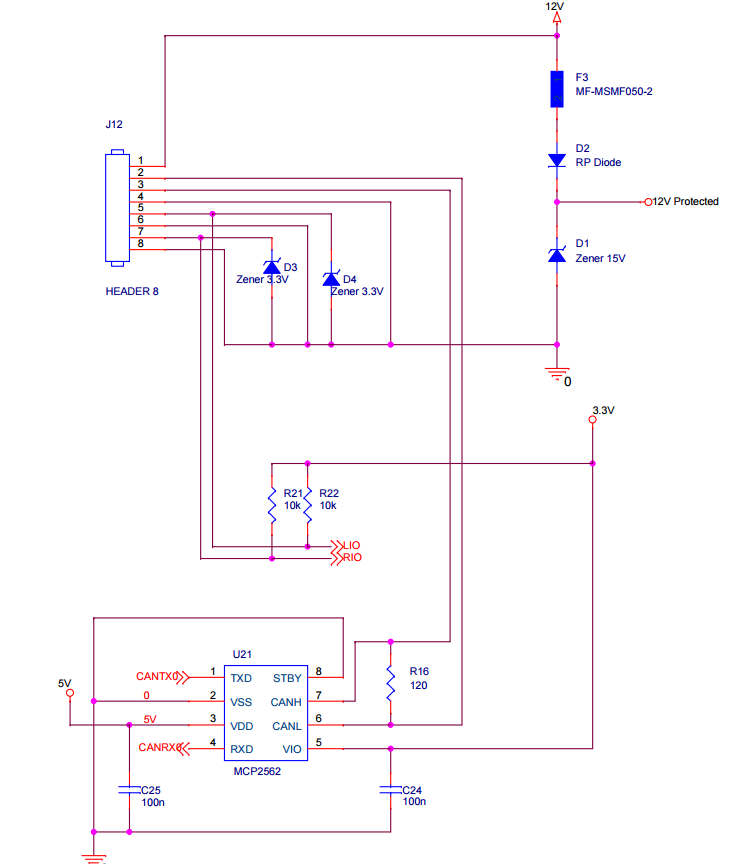
\includegraphics[width=14cm]{Appendices/can.png}
\end{center}
\caption{Circuit diagram of CAN unit.}
\label{fig:can}
\end{figure}


\subsection{Other Components}
\label{sec:other_components}

In order for the device to connect to the car's CAN bus and button inputs, two Bulgin circular connectors were placed on the back, as can be seen in Figure \ref{fig:device_back}. These were chosen for their compactness and they were in accordance to UGR specification. Two connectors were required because the connection to the car and the connection to the steering wheel must be independent for the steering wheel to be removable.

\begin{figure}[H]
\begin{center}
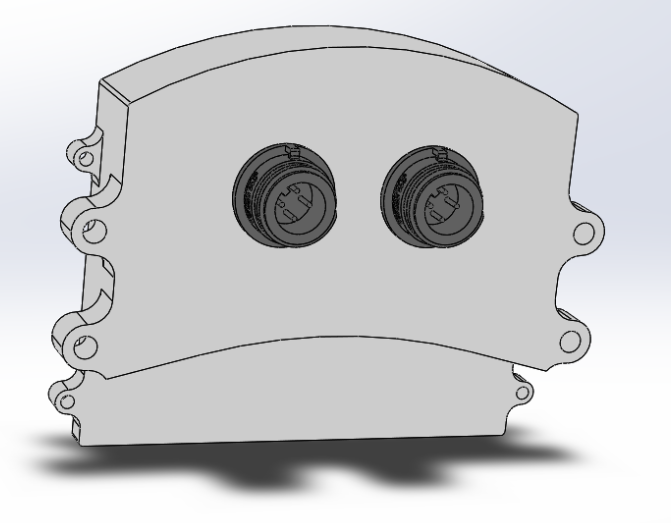
\includegraphics[width=10cm]{Figures/device_back.png}
\end{center}
\caption{Bulgin connectors on the back of the device.}
\label{fig:device_back}
\end{figure}


All other components on the device (resistors, capacitors etc.) were surface mount in order to reduce space on the PCB. The use of 1\% resistors also improved the accuracy of the PSU voltages and other components. \\

% ====================================================================================================================

\newpage
\section{Software Design}
\label{sec:software_design}

As well as the device electronics, the quality of the software is also of high importance in order to ensure the device runs smoothly and meets all of the requirements. As a result, the software needed to be highly maintainable and comprehensive.

\subsection{CAN Software}
\label{sec:CAN_software}

CAN was used throughout the UGR racing car in order to pass information between the different components of the car. The steering wheel display was designed to read the relevant car status information from the CAN bus and output this data on its display at real-time speeds. \\

The CAN software was implemented using the Due CAN library \cite{due_can}. This library is compatible with the Arduino Due board. A large amount of information was sent over the car's CAN bus, however not all of this information was relevant to the device. The role of this software was to filter out the irrelevant information, only sending useful information to the device peripherals. The library allowed various mailboxes to be set up, each with a different CAN identifier (ID), that would call the appropriate function to handle the data in the CAN frame. The LCD screen and RPM LEDs could then be updated with the filtered car information via the display software described in Section \ref{sec:display_software}. \\

The CAN bus requires a set of CAN frame identifiers in order to sort the bus information. Although these CAN identifiers were already specified by UGR, they were subject to change in the future. As a result, these identifiers had to be designed to be configurable on the device. Configurable CAN identifiers were implemented in the diagnostics software using the configuration menu described in Section \ref{sec:configuration_software}.

\subsection{Display Software}
\label{sec:display_software}

The display software was used to output the relevant car information to the device peripherals: LCD display and RPM LEDs. The main requirement of this part of the software was that it had to be clear and easy to read at a glance. As a result, the colour scheme chosen was black and white, and custom fonts were used to improve the visibility of the displayed values. \\

The development of the display software first involved the development of a custom driver for the LCD display. This was designed to allow text and symbols to be output in a specified location on the LCD display, allowing for ease of configurability of the display output when programming. A hierarchy of functions was implemented to abstract away from the low-level commands being issued to the LCD display driver. The hierarchy of functions is demonstrated in Figure \ref{fig:software_hierarchy}. 

\begin{figure}[H]
\begin{center}
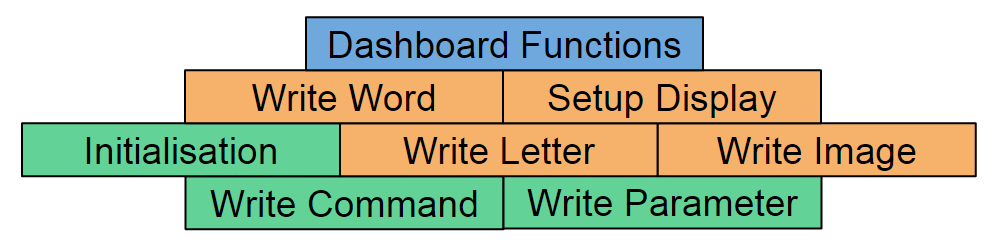
\includegraphics[width=12cm]{Figures/software_hierarchy.png}
\end{center}
\caption{Software Implementation Hierarchy}
\label{fig:software_hierarchy}
\end{figure}


This shows the basic low-level functions at the bottom, defined in the LCD's built-in controller, with more abstract functions implemented by team VoltsWagen above. The middle-layer was built on top of the LCD's built-in controller. Basic functions, allowing text and images to be display anywhere on the screen at specified font sizes were implemented. The top layer describes the main dashboard functions that specifically display the car's status information. This main dashboard software was able to make use of the middle-layer functions to output values onto the LCD display. Figure \ref{fig:display} shows the display software outputting example car information. \\

\begin{figure}[H]
\begin{center}
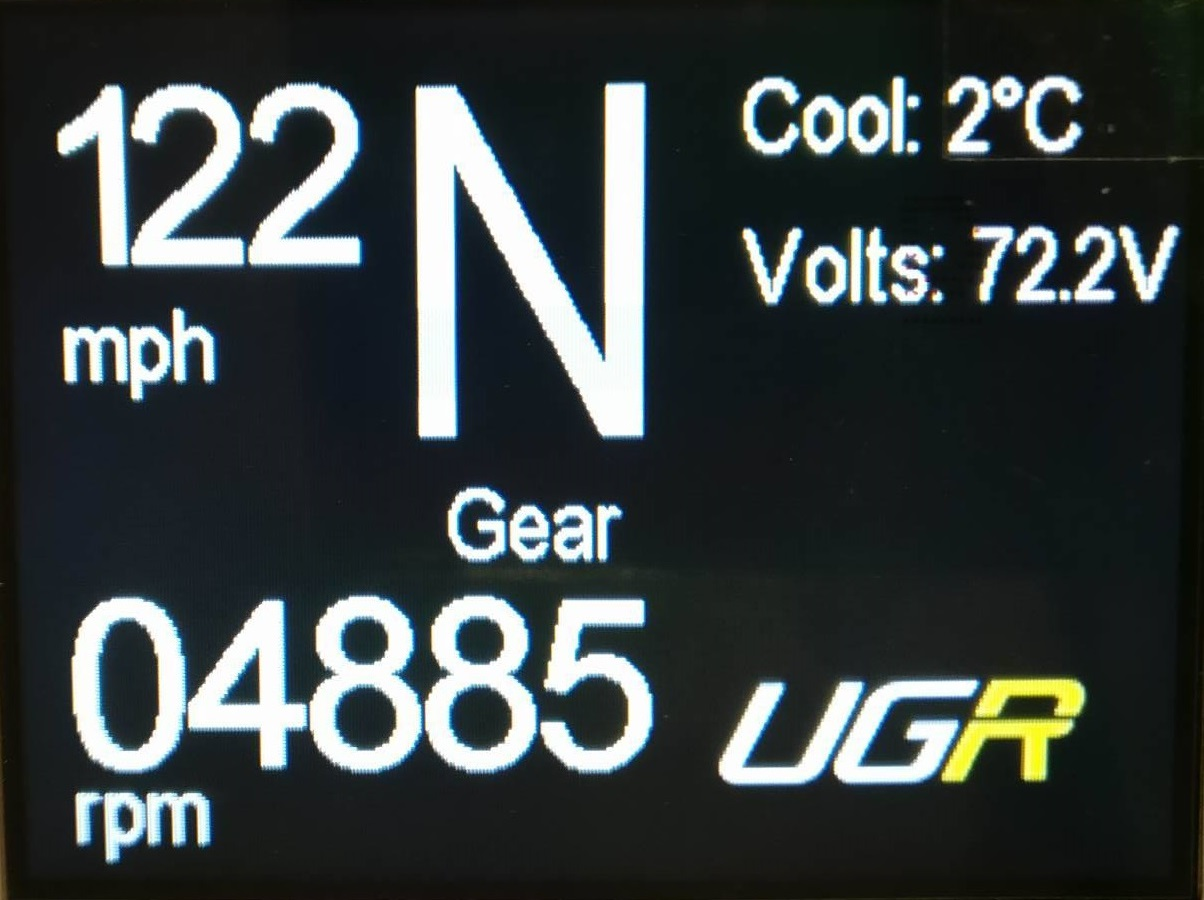
\includegraphics[width=10cm]{Figures/display.jpg}
\end{center}
\caption{Device shown in Display Mode}
\label{fig:display}
\end{figure}


DotStar LEDs were used to display the RPM of the engine, as mentioned in Section \ref{sec:LEDs}. This was implemented in software using the Adafruit DotStar Arduino Library \cite{dotstar_library}, which allowed the colour and brightness of the LEDs to be easily configured.

\subsection{Diagnostics Software}
\label{sec:diagnostics_software}

In order to aid with the debugging of the device with respect to the CAN frames, a Diagnostics Mode was implemented.  When activated, a verbose representation of the CAN bus would be printed onto the LCD display. Figure \ref{fig:diagnostics} shows an example of the CAN diagnostics software in operation. Although this was useful when writing the software, it was also designed to be used by a mechanic for debugging the overall car's CAN bus by allowing the screen to act as a CAN frame probe.

\begin{figure}[H]
\begin{center}
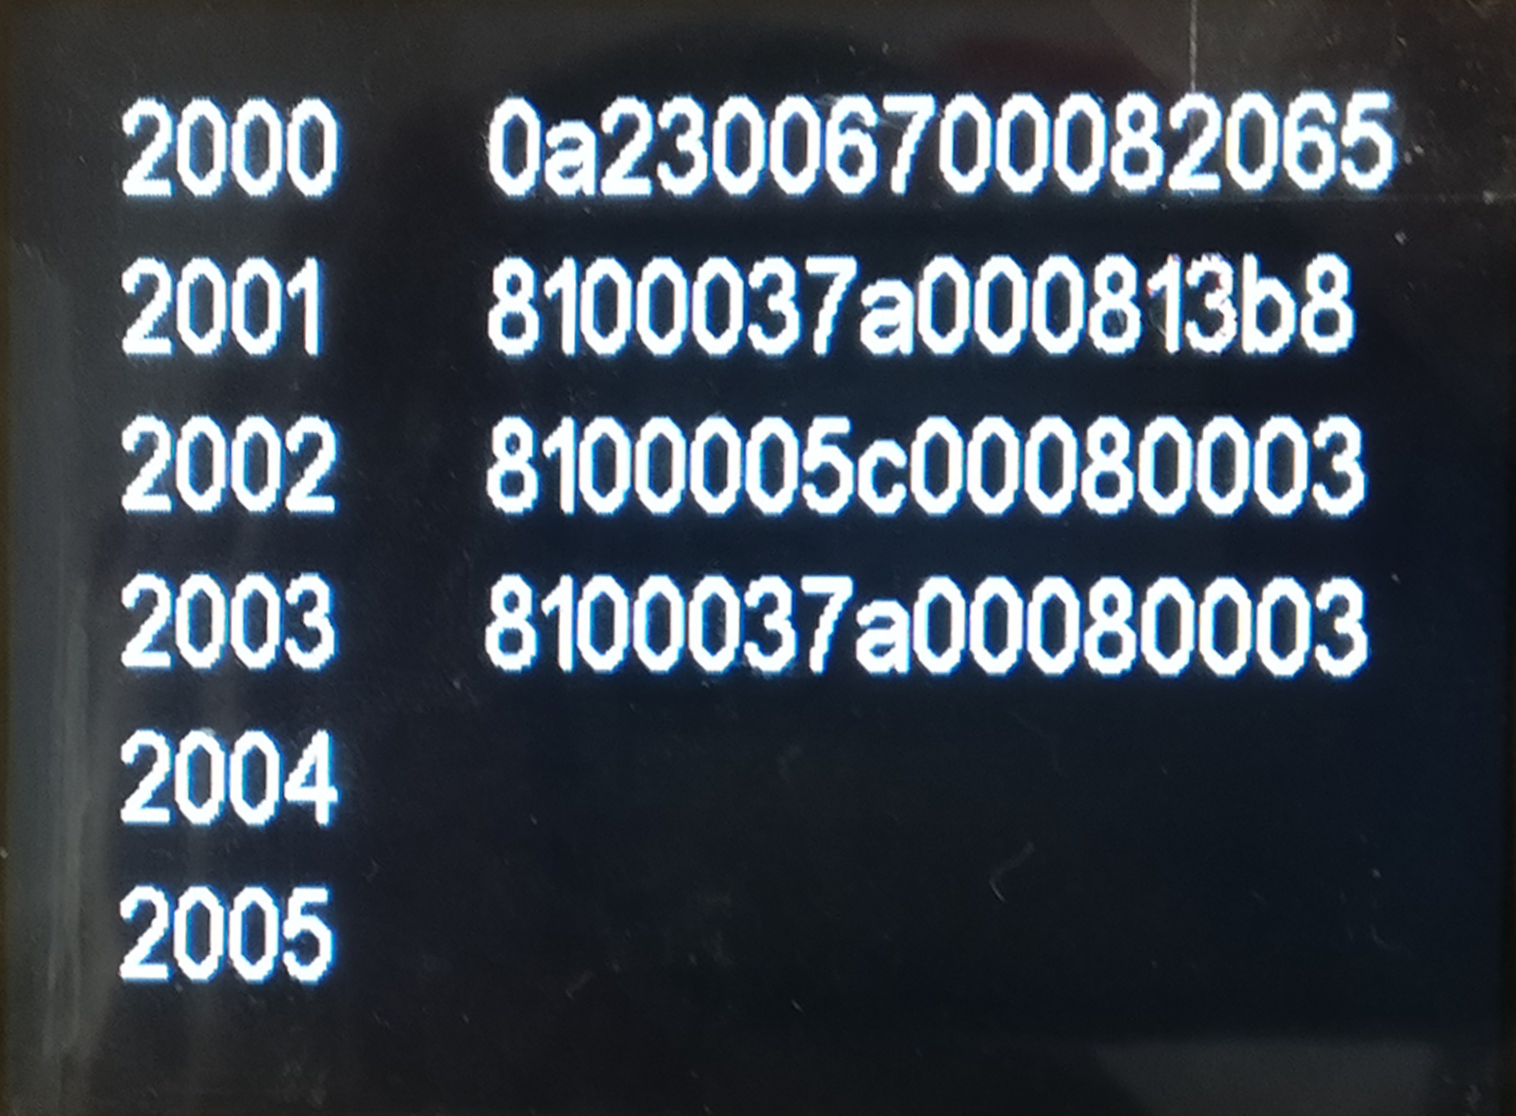
\includegraphics[width=10cm]{Figures/diagnostics.png}
\end{center}
\caption{Device shown in Diagnostics Mode.}
\label{fig:diagnostics}
\end{figure}


Up to 30 different CAN frames were able to be displayed in diagnostics mode. Only 6 CAN frames were to be displayed on the screen at one time, therefore, 6 pages of CAN frames were implemented. The next and previous pages could be viewed by pressing the right and left gear buttons respectively.

\subsection{Configuration Software}
\label{sec:configuration_software}

Some aspects of the device were required by the client to be configurable, as previously discussed. Specifically:

\begin{enumerate}
  \item Threshold for coolant temperature error symbol to show.
  \item Speed units (MPH or KPH).
  \item CAN frame identifiers for use in the diagnostics software.
\end{enumerate}

A configuration menu through Serial USB was therefore implemented. This serial interface allowed the user to configure the various details of the device through a command prompt interface when the device was plugged into a computer. Figure \ref{fig:configuration_software} shows an example of the configuration software being used. The current configuration is printed to the screen, then the user enters the new configuration values when prompted. When the configuration changes are successful, the new configuration is printed to the screen. \\

Further configurability of other elements of the software, such as the layout of the screen, was an option. However it was decided to not implement this because too much flexibility built into a system can make it too complex for the user to use. \\

\begin{figure}[H]
\begin{center}
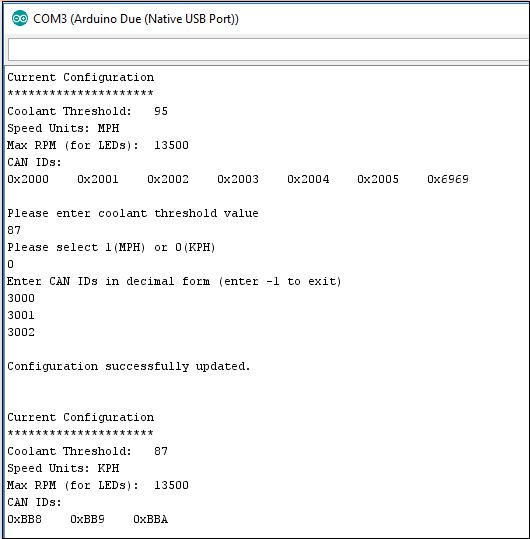
\includegraphics[width=12cm]{Figures/configuration_software.png}
\end{center}
\caption{Example of Configuration Mode in use.}
\label{fig:configuration_software}
\end{figure}


State was stored on the device using the microcontroller's built-in flash memory. This was implemented in software using the Due Flash Storage library \cite{due_flash_storage}. When activated, by plugging the device into a computer with the serial USB port enabled, the user would be able to select personalised configuration options. After configuration the new values would automatically be loaded into the software when the device is next turned on. If the device was not yet configured, then default values are loaded into the software instead.

% ====================================================================================================================

\newpage
\section{Mechanical Design}
\label{sec:mechanical_design}

As well as the electrical components, the device required mechanical design in order to meet the requirements of the UGR team.

\subsection{Outer Enclosure}
\label{sec:outer_enclosure}

In order to house the device components, an outer enclosure needed to be constructed. The requirements from the UGR team are as follows:

\begin{enumerate}
  \item Must mount onto the current UGR wheel.
  \item Must be lightweight.
  \item IP67 Watertight.
  \item Must allow for correct use of the wheel, and therefore be constrained dimensionally.
  \item Must incorporate shifting buttons as they are in the same area of the wheel.
\end{enumerate}

The outer enclosure was developed using SolidWorks, with reference to the steering wheel CAD provided by UGR. An exploded render of the outer enclosure is shown in Figure \ref{fig:device_render_expanded}. This was 3D printed using through the University.

\begin{figure}[H]
\begin{center}
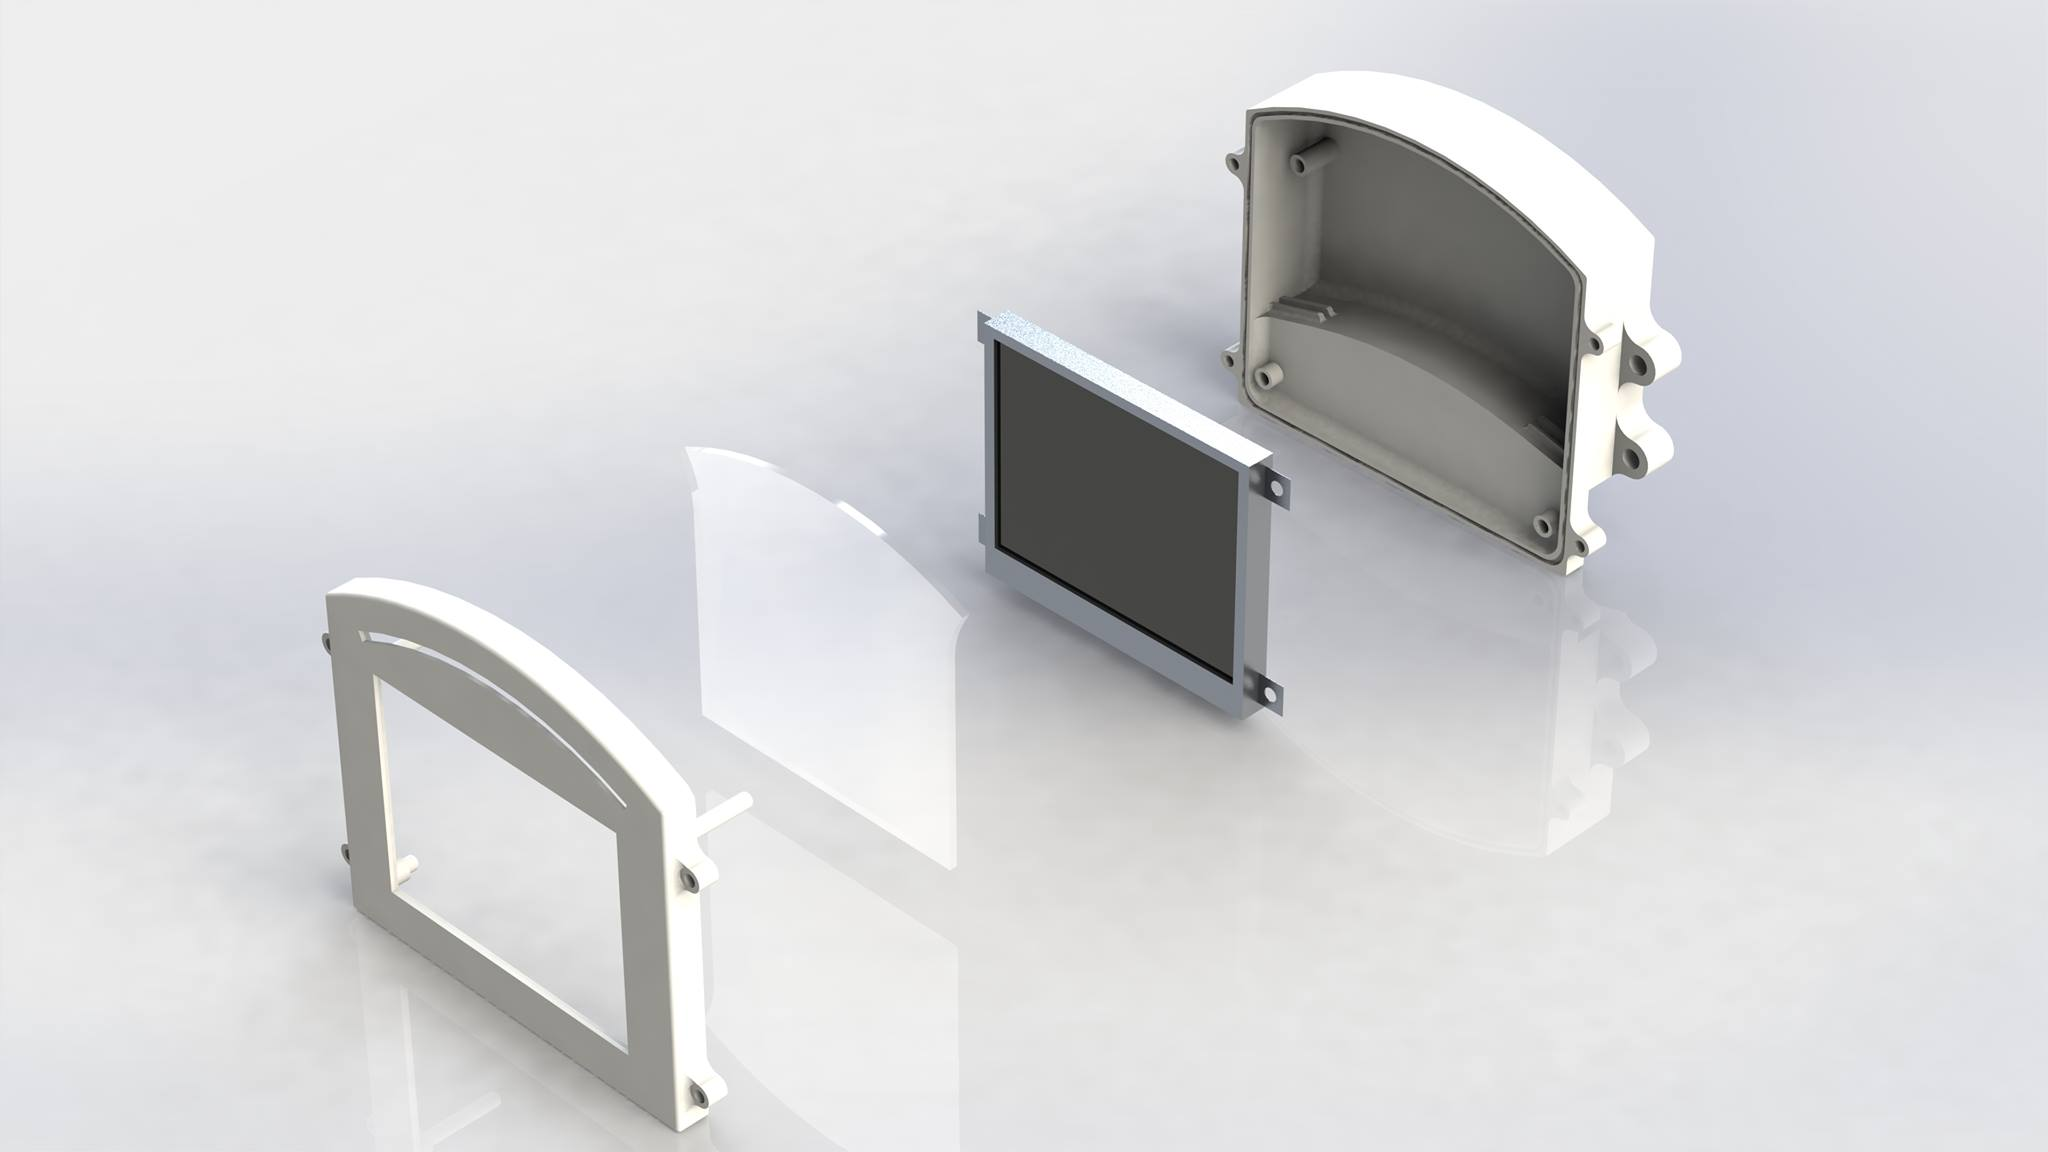
\includegraphics[width=12cm]{Figures/device_render_expanded.jpg}
\end{center}
\caption{SolidWorks render of outer enclosure and display.}
\label{fig:device_render_expanded}
\end{figure}


The enclosure defined the space requirements for all parts enclosed, and how they must fit together. It was decided that the enclosure would be fixed together external to the gaskets to improve watertightness. Unlike design from previous Team Project EE4 teams, the PCB was separated from the screen into a different section of the case, positioned through the top hole of the steering wheel. This decision greatly improved the aesthetics of the device as it was near flush with the front of the steering wheel.

\subsection{Printed Circuit Board}
\label{sec:printed_circuit_board}

As a result of the space constraints, the PCB needed to be able to fit within the design of the outer enclosure. This required the PCB to be of a specific shape, with specific placement of some components (ie. LEDs) as well as a constant awareness of component height, and with the use of small electrical components wherever possible. The shape of the PCB within the context of the outer enclosure is described in Figure \ref{fig:PCB}.

\begin{figure}[H]
\centering
\begin{subfigure}{.5\textwidth}
  \centering
  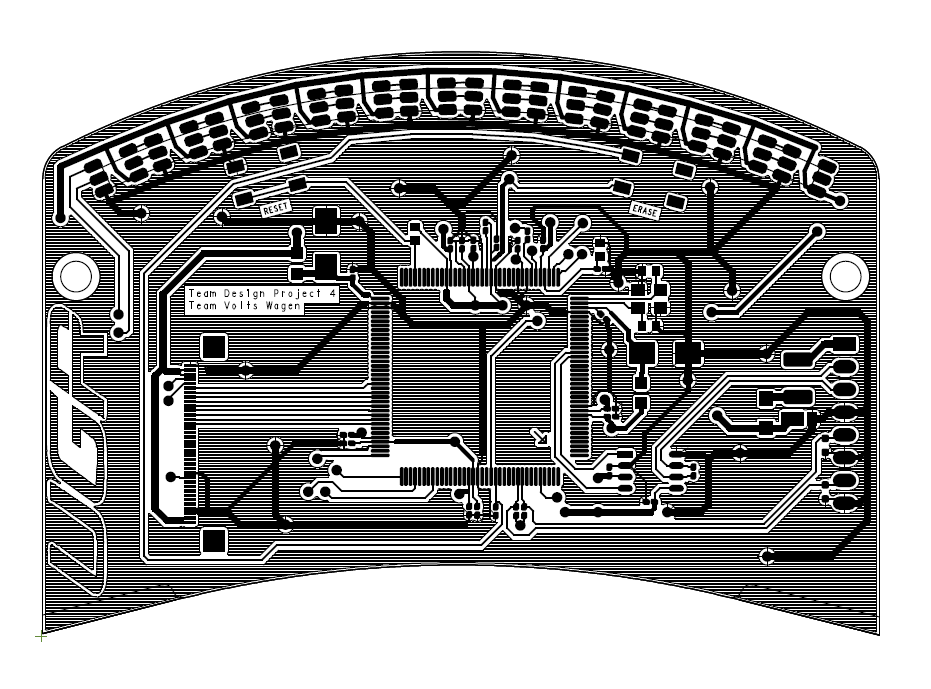
\includegraphics[width=8.5cm]{Figures/PCB_front.png}
  \caption{PCB design front view.}
  \label{fig:PCB_front}
\end{subfigure}%
\begin{subfigure}{.5\textwidth}
  \centering
  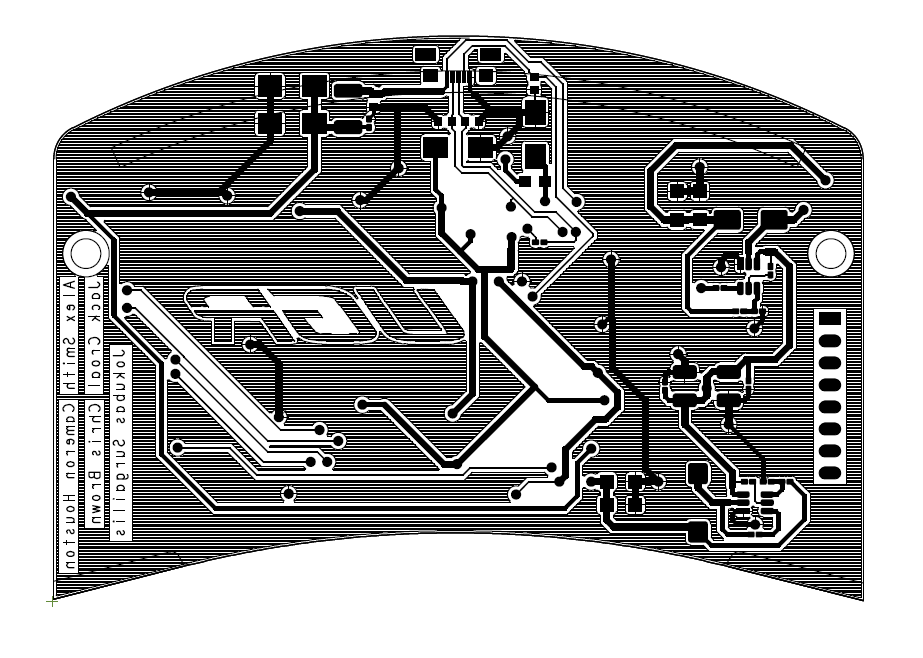
\includegraphics[width=8.5cm]{Figures/PCB_back.png}
  \caption{PCB design rear view.}
  \label{fig:PCB_back}
\end{subfigure}
\caption{Overall PCB design for case.}
\label{fig:PCB}
\end{figure}

% ====================================================================================================================

\newpage
\section{Costs and Expenditure}
\label{sec:cost}

Costs were monitored throughout the design and fabrication of the device. It was important to minimise these costs, without lowering the performance of the device below the expected requirements.

\subsection{Cost for fabrication of the device}
\label{sec:device_cost}

The approximate cost for the materials of the device was \pounds90. The fabrication of the PCB and the outer enclosure are not included in this value because the University services were used. \\

As described in Section \ref{sec:outer_enclosure}, the outer enclosure was developed using a 3D printed plastic. This could have been fabricated out of a different, more expensive, material such as aluminium. This would be expected to improve the heat dissipation, mechanical sturdiness and overall appearance of the device. However, it was decided that the cost trade-off was too high, and the device would still perform well within the requirements if a plastic outer enclosure was used instead.

\subsection{Total cost for development}
\label{sec:total_cost}

As expected, the total cost for the fabrication and design of the device is considerably higher than \pounds90. This is because multiple prototypes were constructed and tested. For example, a large PCB text board was fabricated in order to the all of the components together before implementing this on the official PCB. This allowed for time for debugging and changes before the final board was developed. There were also a number of smaller test PCBs fabricated to allow for the testing of individual sections of the device. \\

The total cost of components is included in Appendix \ref{app:cost}.

% ====================================================================================================================

\newpage
\section{Project Management}
\label{sec:project_management}

This section documents how the team was structured as well as showing how pivotal the planning stage was to the success of the project.

\subsection{Team Roles}
\label{sec:team_roles}

Although there were no specific roles assigned to members of the team, each team member found themselves contributing to specific parts of the project. Basic roles were used to split the project into separate tasks. For example, the software, electrical and mechanical aspects of the design. However, these roles were not rigid and there were crossovers throughout the project. This method worked well and a key part of the success of this setup was due to regular team meetings. This ensured that each team member was aware of the progress that had been made and what each member needed to focus on for the next meeting: established a common understanding. This kept the team on track and ultimately helped in having a fully functional product in time for the deadline.

\subsection{Gantt Chart}
\label{sec:gantt_chart}

In order for the project to succeed it was crucial to develop a Gantt chart that would both help to break tasks down into manageable chunks and also make sure that deadlines during the project would be met. The Gantt chart was updated as the project progressed. Lead and lag times were more accurately factored into the chart once specific design decisions were made. The final Gantt chart can be found in Appendix \ref{app:gantt_chart}.

\subsection{Risk Register}
\label{sec:risk_register}

This was a multi-disciplinary project, with many variables required to get the project device working properly and meeting all of the requirements. In order to mitigate the risk involved, a risk register was developed. This identified many of the project risks, and made sure that the team was keeping them in mind during development. The risk register is included in Appendix \ref{app:risk_register}.

% ====================================================================================================================

\newpage
\section{Future Improvements}
\label{sec:future_improvements}

This section describes any possible improvements that could be made to the final device. These features were not included in the design due to various time and resource constraints. Although the final device met the functional and non-functional requirements presented by the UGR team, we believe these future improvements could further improve the capabilities of the overall device.

\subsection{Professionally Fabricated Board}
\label{sec:future_improvement_1}

The PCB was manufactured in Glasgow University and could have been reduced in size, had it been manufactured externally. This was considered during the project design, however it was decided to not get the PCB professionally made due to the extra cost and the 3 weeks of lead time required for the PCB to be fabricated and sent. A quote of £100 from ‘PCB Train’ was obtained \cite{pcb_train}. Making use of the facilities within the University reduced the project risk because it allowed PCBs to be re-designed and fabricated within a short timeframe (1-4 days, compared to the 2-week quote for a professionally made PCB).

% ====================================================================================================================

\section{Conclusion}
\label{sec:conclusion}

The project was a success. All of the requirements from UGR were met, and the final device will be implemented in the UGR racing car this year. Flexibility and configurability was built in to the device which will allow it to continue operation on many UGR cars to come. By the end of the project the device was in full working condition and had been tested rigorously in a laboratory environment. The real test will be when UGR takes the device out on the track at the Silverstone Circuit for the Formula Student 2017 competition. Overall, this project has allowed the team to apply knowledge learned from previous lecture courses to a real development environment, which was a valuable opportunity.

% ====================================================================================================================

\newpage
\bibliographystyle{ieeetr}
\bibliography{bibliography}

% ====================================================================================================================

\addtocontents{toc}{\protect\newpage}
\begin{appendices}

\section{Circuit Diagram}
\label{app:circuit_diagram}

\subsection{CAN and button inputs}
\label{app:can}
\begin{figure}[H]
\begin{center}
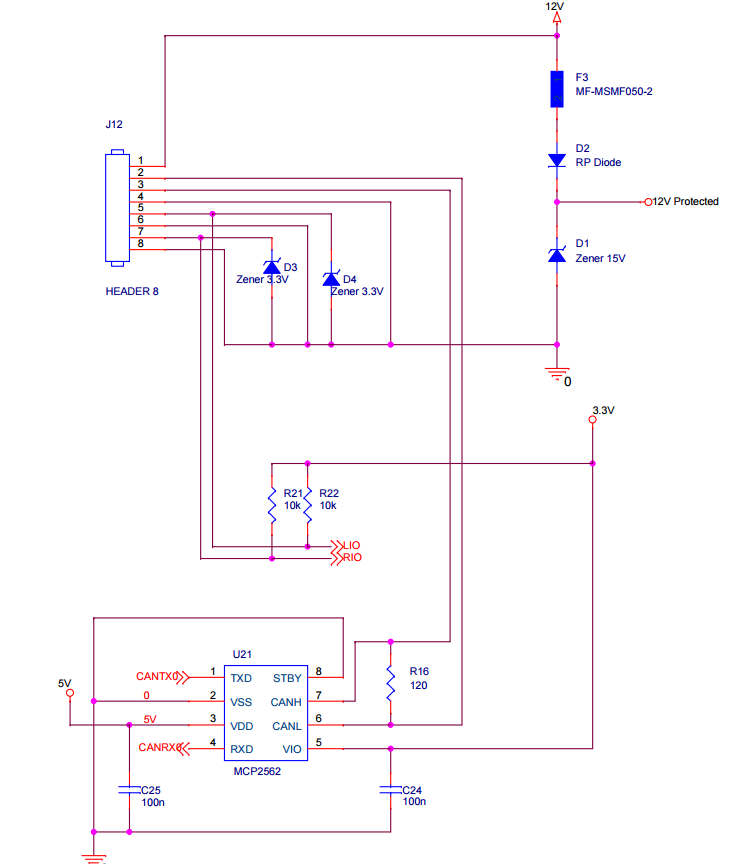
\includegraphics[width=14cm]{Appendices/can.png}
\end{center}
\caption{Circuit diagram of CAN unit.}
\label{fig:can}
\end{figure}


\subsection{Microcontroller and Display}
\label{app:microcontroller}
\begin{figure}[H]
\begin{center}
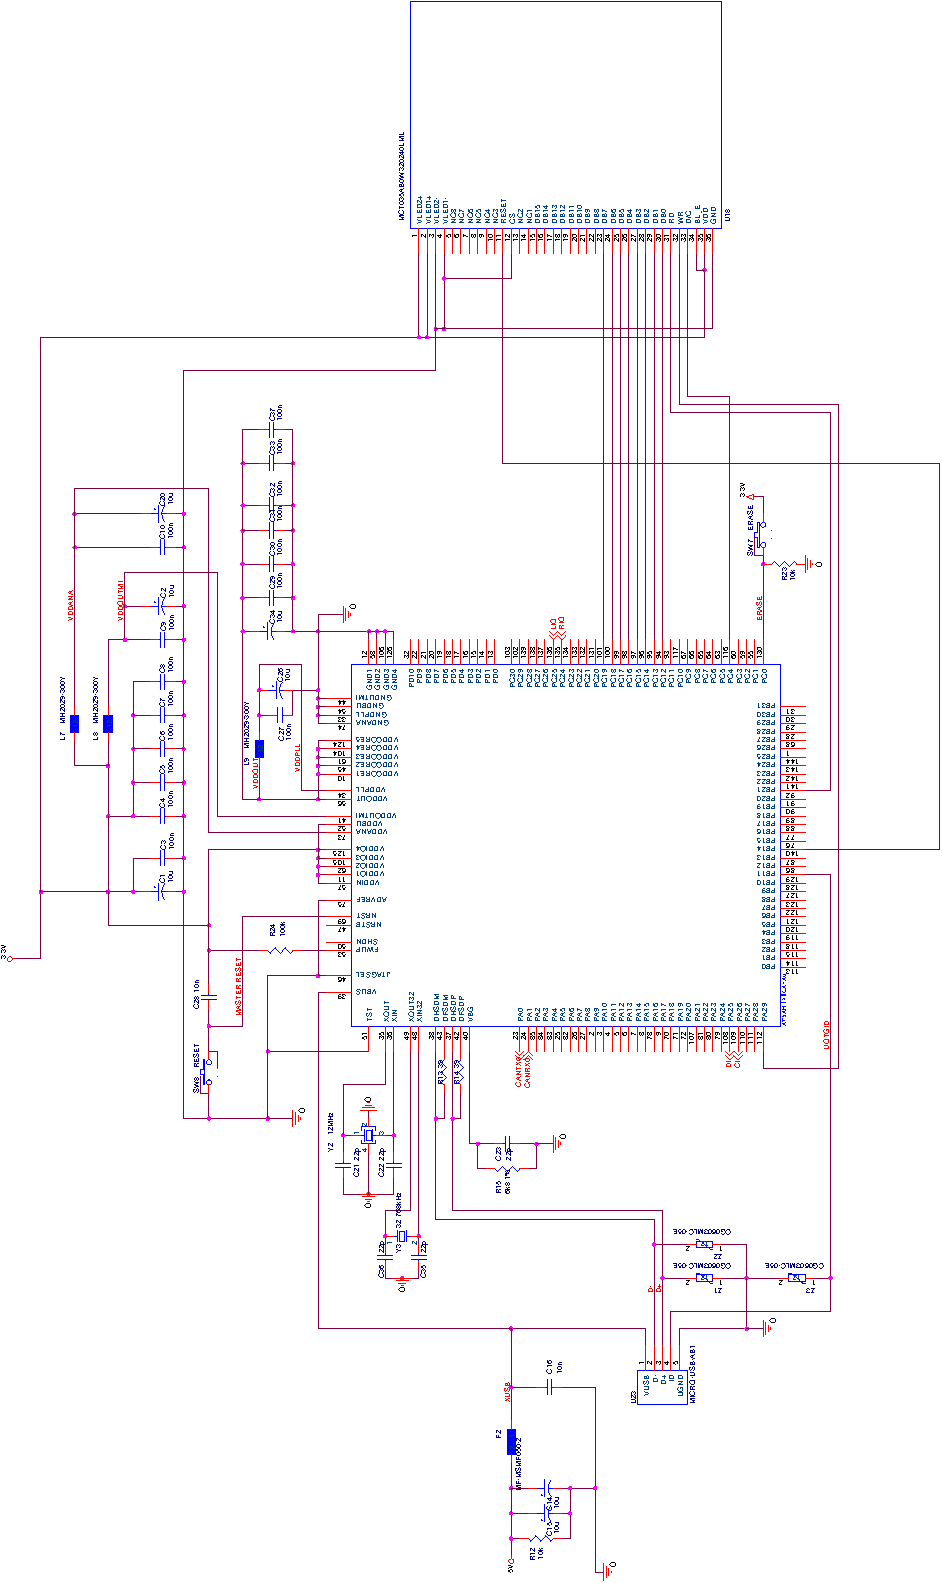
\includegraphics[width=13.5cm]{Appendices/microcontroller_rotated.pdf}
\end{center}
\end{figure}


\subsection{RPM Gauge}
\label{app:leds}
\begin{figure}[H]
\begin{center}
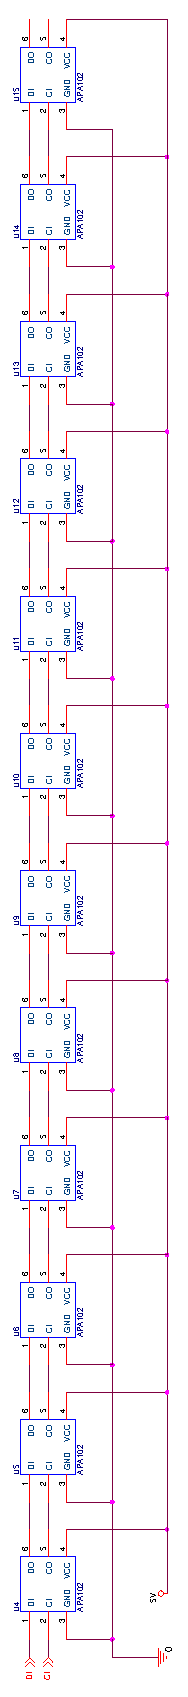
\includegraphics[width=2.4cm]{Appendices/LEDs_full.pdf}
\end{center}
\end{figure}


\subsection{Power Supply Unit}
\label{app:psu}
\begin{figure}[H]
\begin{center}
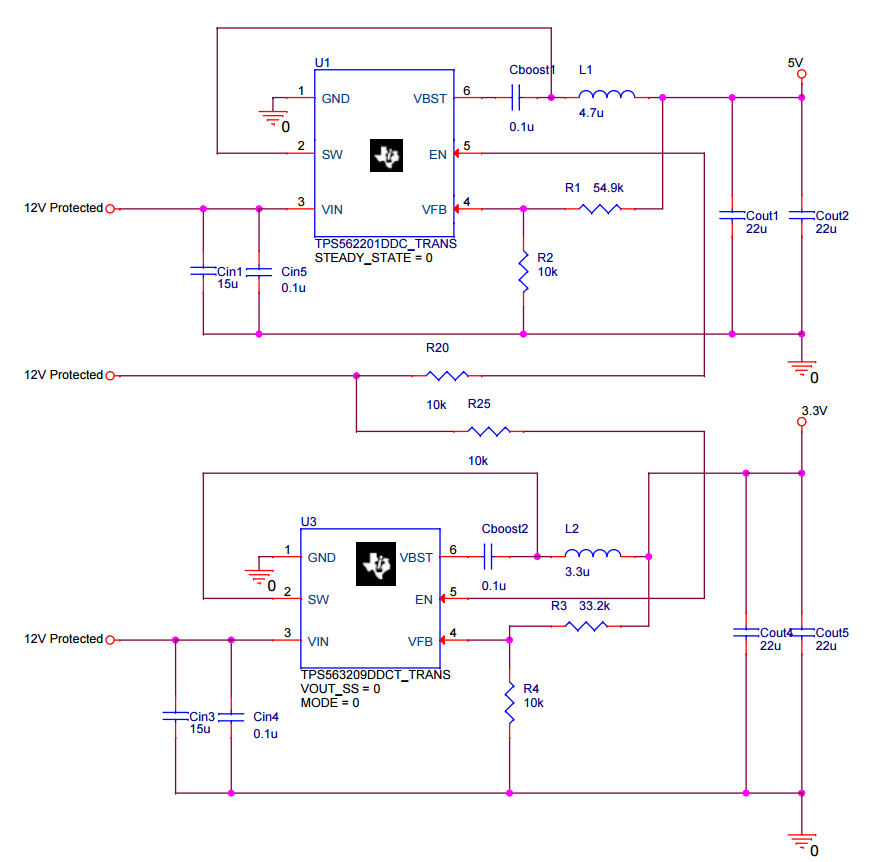
\includegraphics[width=16cm]{Appendices/psu.png}
\end{center}
\end{figure}


\section{Total Component Cost}
\label{app:cost}
\begin{figure}[H]
\begin{center}
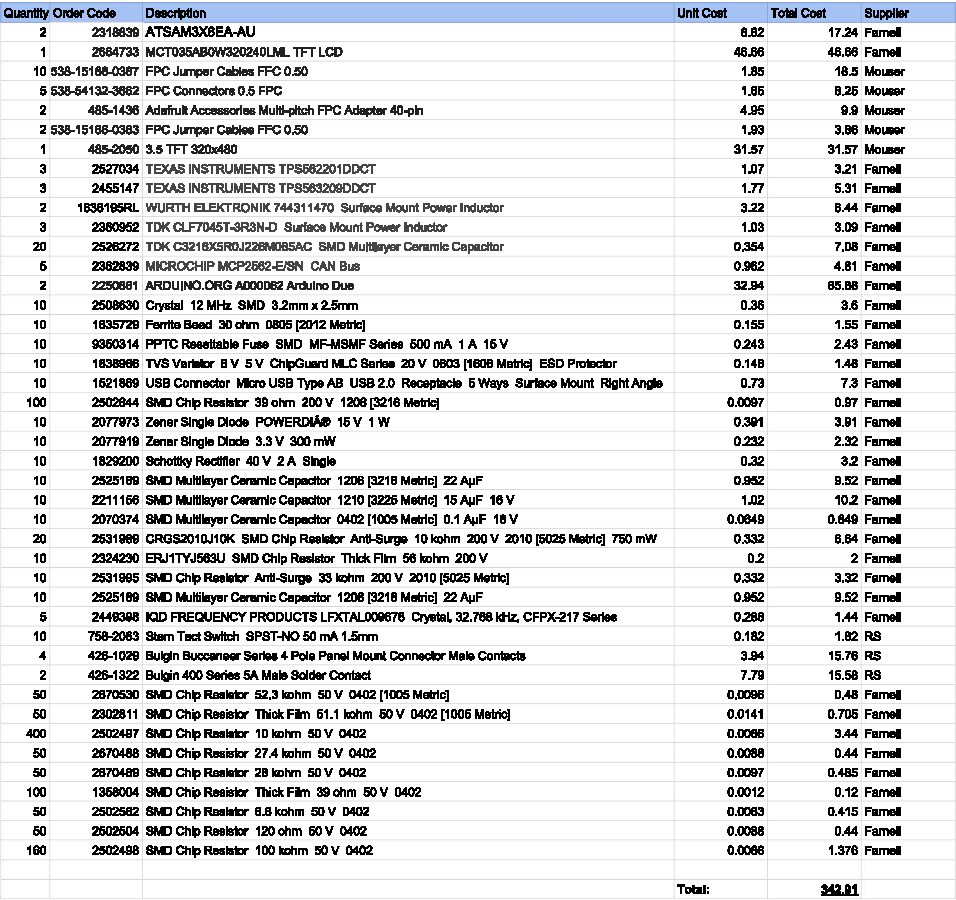
\includegraphics[width=17cm]{Appendices/cost_sheet.pdf}
\end{center}
\end{figure}


\section{Gantt Chart}
\label{app:gantt_chart}
\vspace{-2.5cm}
\begin{figure}[H]
\begin{center}
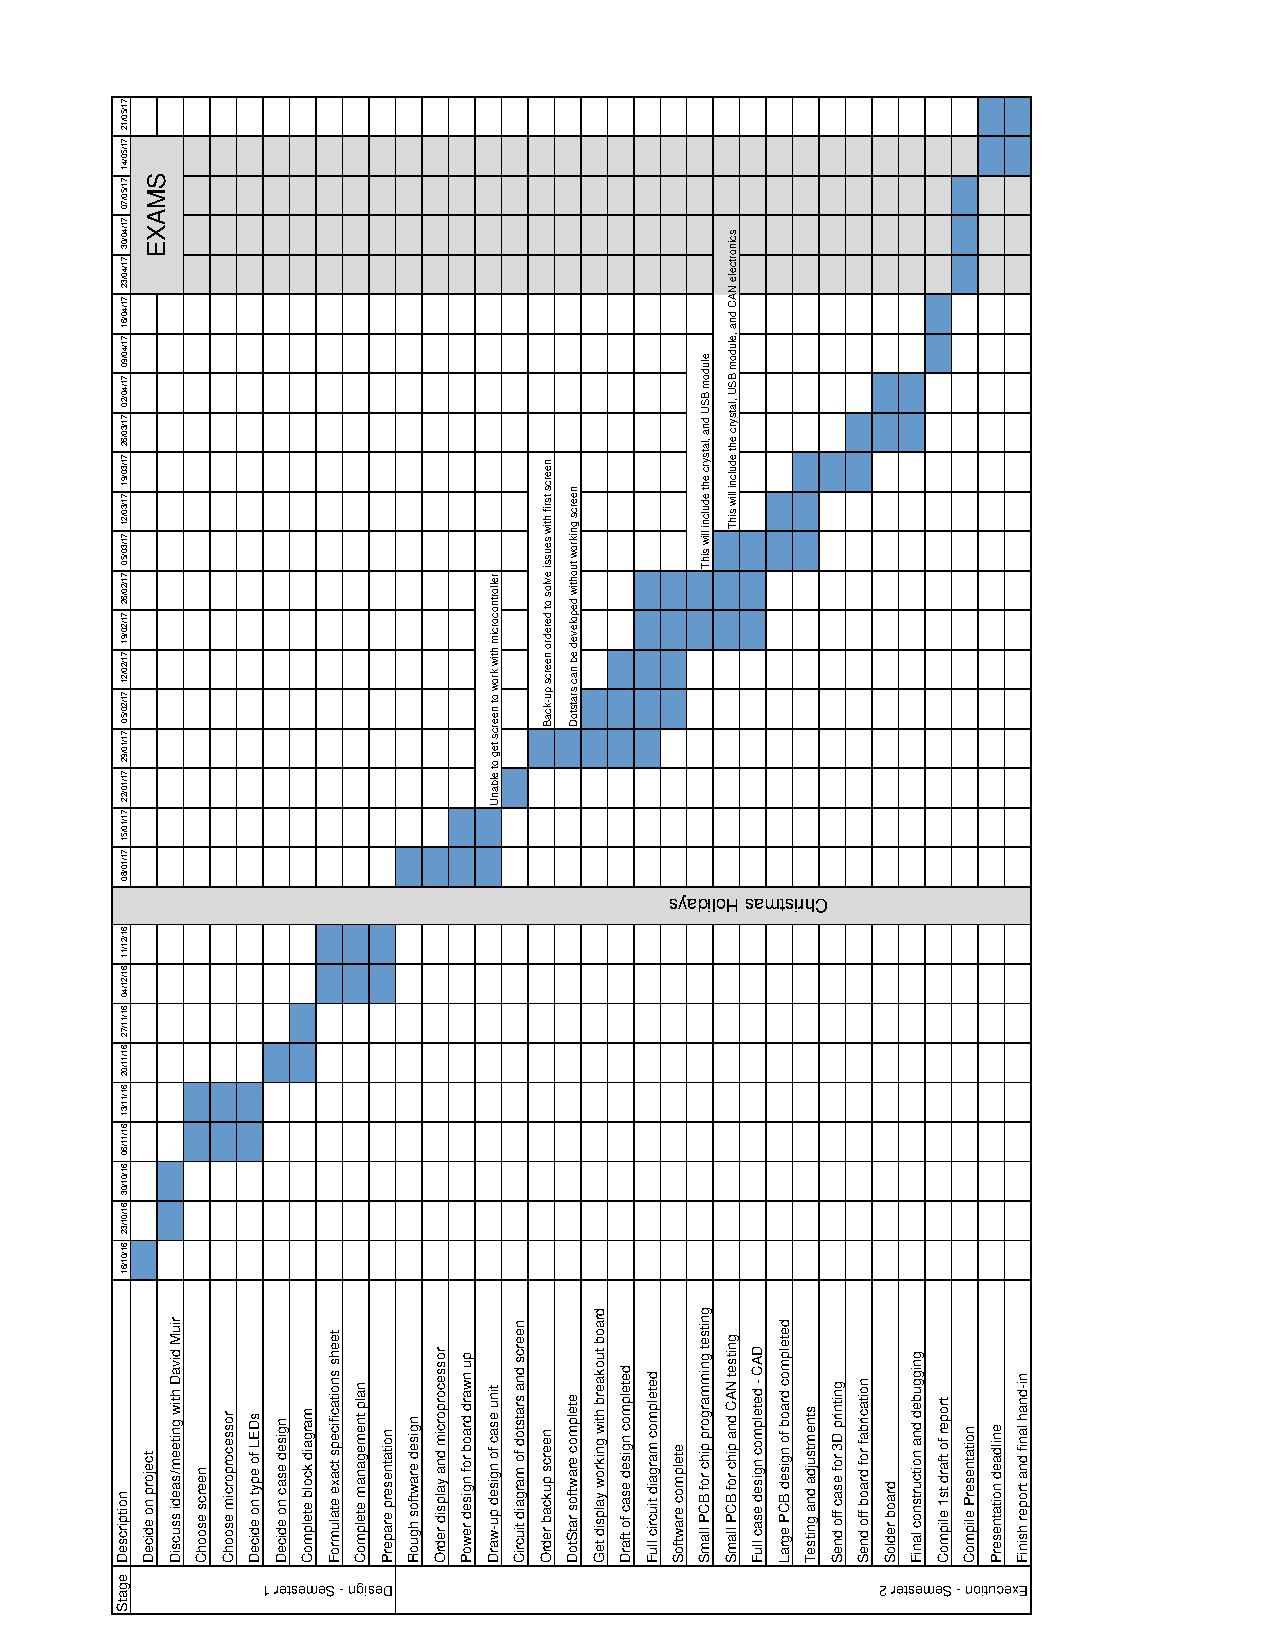
\includegraphics[width=19cm]{Appendices/gantt_chart_rotated.pdf}
\end{center}
\end{figure}


\section{Risk Register}
\label{app:risk_register}
\begin{figure}[H]
\begin{center}
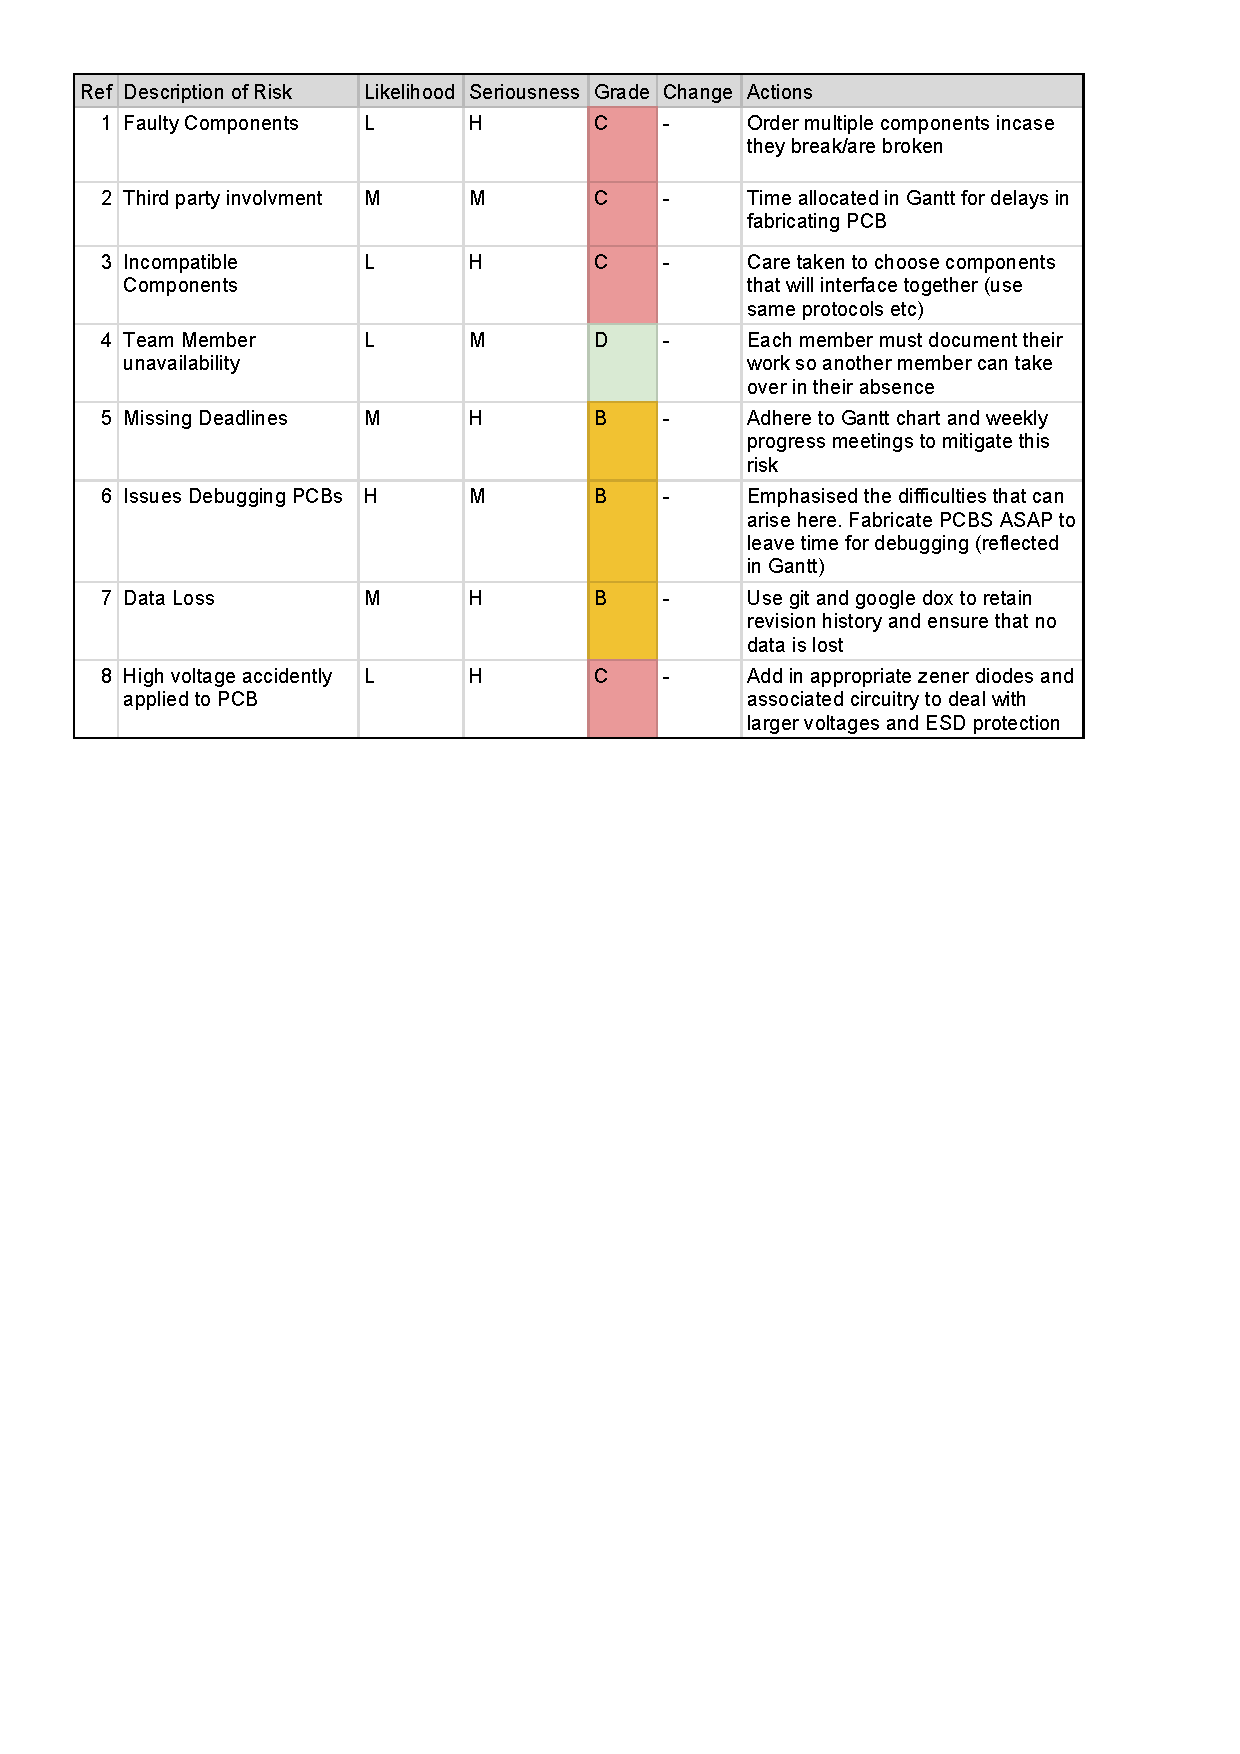
\includegraphics[width=14cm]{Appendices/risk_register.png}
\end{center}
\end{figure}


\end{appendices}

% ====================================================================================================================

\end{document}

































